\documentclass{bioinfo}
\copyrightyear{2013}
\pubyear{2013}

\begin{document}
\firstpage{1}

\title[iview]{iview: WebGL Visualizer of Protein-Ligand Complex}
\author[Hongjian Li \textit{et~al}]{Hongjian Li\,$^{1,}$\footnote{to whom correspondence should be addressed}, Takanori Nakane\,$^{2}$, Kwong-Sak Leung\,$^{1}$ and Man-Hon Wong\,$^{1}$}
\address{$^{1}$Department of Computer Science and Engineering, Chinese University of Hong Kong, Hong Kong\\
$^{2}$Graduate School of Medicine, Kyoto University, Japan}

\history{Received on XXXXX; revised on XXXXX; accepted on XXXXX}

\editor{Associate Editor: XXXXXXX}

\maketitle

\begin{abstract}

\section{Motivation:}
Visualization of protein-ligand complex plays an important role in elaborating protein-ligand interactions and aiding novel drug design. Most existing web visualizers are either too complicated to use, or lack virtual reality support. The feature of macromolecular surface construction is also missing.

\section{Results:}
We have developed iview, an easy-to-use interactive WebGL visualizer of protein-ligand complex, featuring special effects in virtual reality settings and four surface representations. Moreover, we have also developed a neat and tailor-made version specifically for our own istar web platform for bioinformatics and chemoinformatics.

\section{Availability:}
http://istar.cse.cuhk.edu.hk/iview

\section{Contact:} \href{JackyLeeHongJian@Gmail.com}{JackyLeeHongJian@Gmail.com}, \href{nakane.t@gmail.com}{nakane.t@gmail.com}
\end{abstract}

\section{Introduction}

Visualization of protein-ligand complex plays an important role in elaborating protein-ligand interactions and aiding novel drug design. To date, dozens of visualization tools already exist. VMD \citep{1220}, PyMOL \citep{1221} and Chimera \citep{1219} are very well-known and highly cited. They can interpret multiple file formats and generate multiple representations to supply precise and powerful control. AutoDockTools4 \citep{596} provides native support for the PDBQT file format, which is widely used in various protein-ligand docking software such as AutoDock \citep{596}, AutoDock Vina \citep{595}, and our idock \citep{1153}. A case study \citep{1321} is presented to process large amounts of geometry data for real-time 3D exploration, superimposition, and interactive navigational tasks in a virtual reality environment. We also developed our own method \citep{1265} to visualize structures in virtual reality settings and employ fragment-based \textit{de novo} ligand design strategy for interactive drug design. PoseView \citep{748} and LigPlot+ \citep{951}, on the other hand, plot 2D diagrams of protein-ligand interactions from 3D coordinates.

In addition, there are web visualizers based on either Java applet, Adobe Flash, or HTML5 canvas. Jmol (http://www.jmol.org), an open source Java viewer for chemical structures in 3D, has been deployed worldwide and recognized as the \textit{de facto} molecular viewer on the web. JSmol \citep{1314}, a JavaScript-only version of Jmol, includes the full implementation of the entire set of Jmol functionalities. GLmol (http://webglmol.sourceforge.jp), a molecular viewer on WebGL/Javascript using the three.js library, supports multiple file formats and representations, and features an experimental version of surface construction based on the EDTSurf algorithm \citep{1297}. Another study \citep{1262} also presents a WebGL technology for rendering molecular surface using the SpiderGL library \citep{1320}. ChemDoodle Web Components (http://web.chemdoodle.com), a pure Javascript chemical graphics and cheminformatics library, presents 2D and 3D graphics and animations for chemical structures, reactions and spectra. ePlant \citep{1242}, a suite of open-source Flash-based web tools, visualizes integrative systems biology from the model organism \textit{Arabidopsis thaliana}. PLI \citep{1288} is a web-based tool for the comparison of protein-ligand interactions observed on PDB structures. BioJS \citep{1308} is an open source JavaScript framework for biological data visualization. There is a review that covers a history of web-based structure input \citep{1243}.

Surface representation is a convenient way to visualize protein-ligand interactions. However, macromolecular surface calculation is computationally and memory intensive. Furthermore, the calculated mesh is very complex, often exceeding 500,000 polygons. Therefore its implementation in Javascript/WebGL was considered to be very difficult. On one hand, most existing web visualizers are either too complicated to use, or lack virtual reality support. On the other hand, the feature of surface construction is missing.

To address the above obstacles, we were inspired by ChemDoodle Web Components and GLmol, and have thus developed iview, an easy-to-use interactive WebGL visualizer of protein-ligand complex, featuring special effects in virtual reality settings and four surface representations. Furthermore, we have recently developed a web platform called istar in order to automate large-scale protein-ligand docking using our idock \citep{1153}. Apart from the feature-rich version of iview, we have also developed a neat and tailor-made version specifically for visualizing docking results of user-submitted jobs.

%Modern browsers nowadays, e.g. Chrome, Firefox, Safari and Opera, support WebGL. IE11 will support WebGL too.

\begin{methods}
\section{Methods}

iview is refactored from GLmol 0.47, using three.js as its primary 3D engine with antialias support. It can be easily integrated into HTML5 web pages to display molecular models without requiring Java or plugins. It loads a protein-ligand structure from the PDB (Protein Data Bank) \citep{539,537} as its data source via a RESTful interface. It renders four standard representations of primary structure, namely line, stick, ball \& stick and sphere, and five standard representations of secondary structure, namely ribbon, strand, cylinder \& plate, C alpha trace and B factor tube. It colors the structure by either atom spectrum, protein chain, protein secondary structure, B factor, residue name, residue polarity, or atom type, by setting the vertex colors of the geometry object of the corresponding representation. It supports user interactions including rotation, translation, zooming and slabing with mouse or hand touch manipulation. It provides both perspective and orthographic cameras, and both anaglyph and parallax barrier effects from three.js examples for use in a virtual reality environment. When users wear a spectacle with special filters on both sides, the disparity between two superimposed molecules creates a perception of depth, leading to visually more appealing identification of intermolecular interactions.

We have ported EDTSurf \citep{1297}, an fast algorithm to generating triangulated macromolecular surfaces by Euclidean distance transform, to Javascript and integrated it into iview to construct and render four representations of protein surface, namely Van der Waals surface, solvent excluded surface, solvent accessible surface and molecular surface, with opacity and wireframe adjustable by users. Although the Javascript implementation of the EDTSurf algorithm typically consumes a few seconds and 500MB to 700MB memory for computation, it is sufficiently efficient for practical applications. To limit CPU and memory usage, the calculation grid size is restricted to 180 x 180 x 180.

Based on the feature-rich version, the tailor-made version of iview specifically for idock jobs removes the majority of dispensable functions and therefore shapes a very neat interface. It only retains the rendering of primary structure of protein and ligand in four representations, as well as the construction of protein surface. Most importantly, it implements additional features. It displays the user-supplied search space in the form of a cubic box so that the binding site is visually depicted. Its parsers are capable of parsing a protein and multiple top hit ligands in PDBQT format as used by idock. It displays the top hit ligand IDs in a horizontally scrollable row and provides a straightforward way to switch ligands easily. It lists the docking result files, predicted binding affinity values, molecular properties, compound suppliers and annotations, and putative hydrogen bonds, in order to give users a quick overview of the top hit ligands, and assist them in making decisions of which compounds to purchase for subsequent wet-lab experiments.

\end{methods}

\section{Results}

4MBS \citep{1348}

\begin{figure}%[!tpb]
\centerline{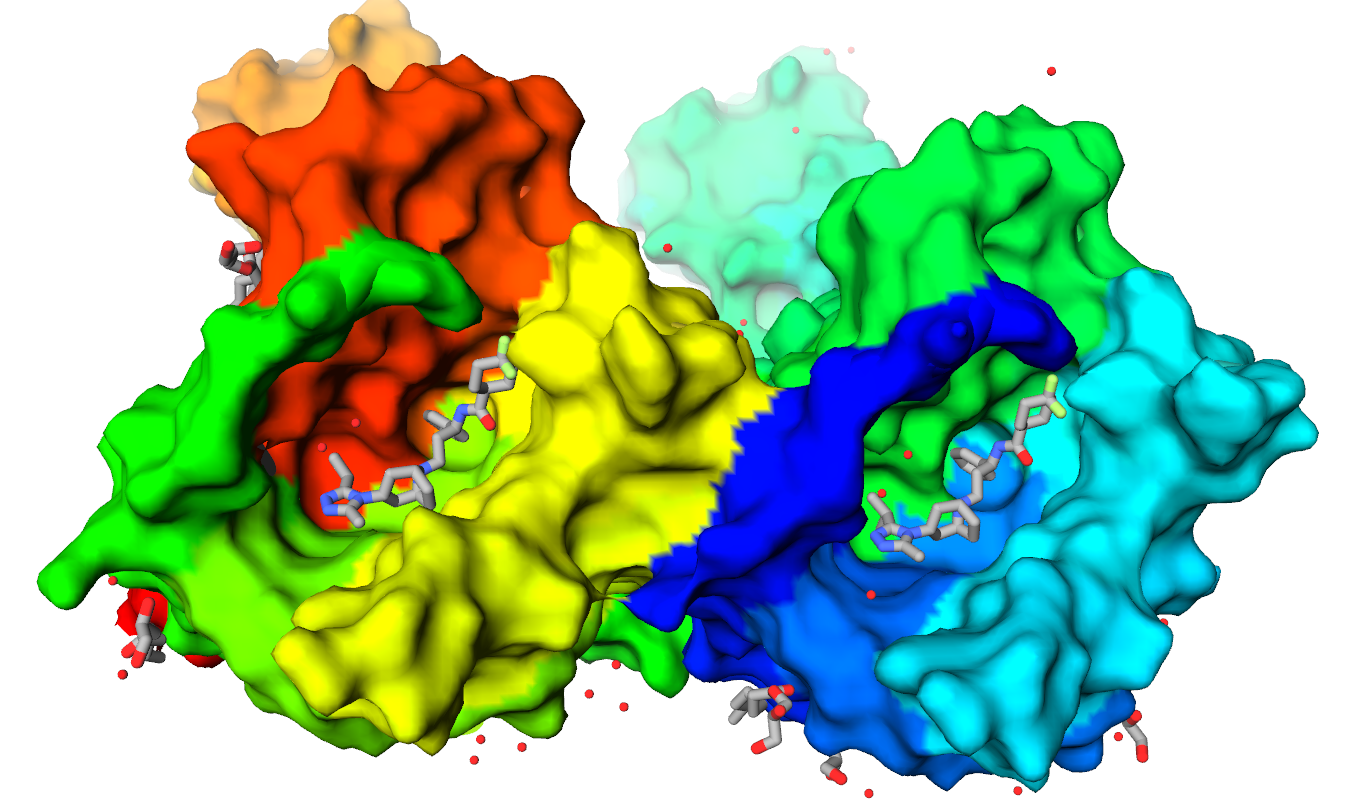
\includegraphics[width=\linewidth]{4MBS.png}}
\caption{iview rendering of the CCR5 chemokine receptor-HIV entry inhibitor maraviroc complex (PDB code: 4MBS). The human CCR5 is rendered as molecular surface colored by spectrum. The marketed HIV drug maraviroc is rendered as stick colored by atom types. It can be clearly seen that the CCR5 forms a deep allosteric cavity where maraviroc is buried.}\label{fig:4MBS}
\end{figure}

\section{Availability}

iview is free and open source under Apache License 2.0. iview is available at http://istar.cse.cuhk.edu.hk/iview. Its source code is available at https://github.com/HongjianLi/istar.

%\section{Conclusion}

%We have developed iview, an interactive WebGL visualizer of protein-ligand complex. Manipulate ligands only. Text rendering. Visual docking. Rescoring with RF-Score.

\bibliographystyle{natbib}
%\bibliographystyle{achemnat}
%\bibliographystyle{plainnat}
%\bibliographystyle{abbrv}
%\bibliographystyle{bioinformatics}
%
%\bibliographystyle{plain}

\bibliography{../refworks}

\end{document}
